% !TeX program = xelatex
% !TeX encoding = UTF-8

\documentclass[UTF8,a4paper,zihao=-4]{ctexart}

% =========================================================
% 页面设置
% =========================================================
\usepackage{geometry}
\geometry{
  left=2.6cm,
  right=2.6cm,
  top=2.8cm,
  bottom=2.8cm
}

\usepackage{setspace}
\onehalfspacing

\usepackage{indentfirst}
\setlength{\parindent}{2em}

% =========================================================
% 数学与符号
% =========================================================
\usepackage{amsmath}
\usepackage{amssymb}
\usepackage{bm}

% =========================================================
% 图表
% =========================================================
\usepackage{graphicx}
\usepackage{float}
\usepackage{subcaption}
\usepackage{booktabs}
\usepackage{array}
\usepackage{multirow}

% 图片路径
\graphicspath{{figures/}}

% =========================================================
% 单位与数字
% =========================================================
\usepackage{siunitx}
\sisetup{
  detect-all,
  separate-uncertainty = true
}

% =========================================================
% 列表与代码
% =========================================================
\usepackage{enumitem}
\usepackage{xcolor}
\usepackage{listings}

\lstset{
  basicstyle=\ttfamily\small,
  breaklines=true,
  frame=single,
  columns=fullflexible,
  numbers=left,
  numberstyle=\tiny,
  keywordstyle=\bfseries,
  commentstyle=\itshape,
  showstringspaces=false
}

% =========================================================
% 超链接
% =========================================================
\usepackage[
  colorlinks=true,
  linkcolor=black,
  citecolor=black,
  urlcolor=blue
]{hyperref}

% =========================================================
% 参考文献
% =========================================================
\usepackage[backend=biber,style=gb7714-2015]{biblatex}
\addbibresource{refs/references.bib}

% =========================================================
% 标题格式
% =========================================================
\ctexset{
  section = {
    format = \Large\bfseries,
    name = {,、},
    number = \chinese{section}
  },
  subsection = {
    format = \large\bfseries
  },
  subsubsection = {
    format = \normalsize\bfseries
  }
}

% =========================================================
% 自定义命令
% =========================================================
\newcommand{\snr}{\mathrm{SNR}}
\newcommand{\mfcc}{\mathrm{MFCC}}
\newcommand{\stft}{\mathrm{STFT}}
\newcommand{\fft}{\mathrm{FFT}}

% =========================================================
% 文档信息
% =========================================================
\title{\heiti 基于信号处理的孤立数字语音识别实验报告}

\author{
  于沛龙 \quad 景序 \quad 封宇凡 \quad 孟德轩
}

\date{2026年5月}

% =========================================================
% 正文
% =========================================================
\begin{document}

\maketitle

\begin{abstract}
本实验面向数字 0--9 的孤立词语音识别任务，
基于 7 位说话人共 70 段语音（训练集 speaker1--5 共 50 条，
验证集 speaker6--7 共 20 条），
完成了语音信号分析、MFCC 特征提取、分类识别和噪声鲁棒性测试。
在信号处理方面，对语音进行端点检测、预加重、分帧加窗和短时傅里叶分析，
提取 13 维 MFCC 及其一阶、二阶动态差分特征（共 39 维）。
在分类方面，分别采用基于 26 维统计特征的 KNN 基线、
基于 39 维帧级序列特征的 GMM 模型以及基于 MFCC 动态特征图的卷积神经网络（CNN）进行数字分类。
实验结果表明，纯净语音条件下 GMM 与 CNN 均达到 100.0\% 识别准确率；
在混合噪声（白噪声、1/f 粉红噪声与 50 Hz 工频干扰）条件下，各模型识别性能随信噪比降低而下降，
其中 GMM 是传统方法中最稳定的方案，CNN 在中高 SNR 区间保持了较好的识别性能。
实验验证了信号处理方法在语音识别中的有效性，同时也揭示了小样本数据集下不同方法的优劣与局限。
\end{abstract}

\noindent\textbf{关键词：}
孤立词语音识别；MFCC；KNN；GMM；CNN；噪声鲁棒性；信号与系统

\newpage

\tableofcontents

\newpage

本实验面向数字 0--9 的孤立词语音识别任务，
完成了从数据预处理、信号分析、特征提取、模型训练到噪声鲁棒性测试的完整流程。
实验首先对语音信号进行端点检测、预加重、分帧加窗和短时傅里叶分析，
并提取梅尔频率倒谱系数（MFCC）及其动态特征。
随后，分别采用 MFCC 统计特征结合 KNN、MFCC 序列特征结合 GMM，
以及基于 MFCC 动态特征图的 CNN 模型进行数字分类。
实验结果表明，在纯净语音条件下，GMM 方法取得了较高识别准确率；
在混合噪声条件下，识别性能随信噪比降低而下降。
通过对时域、频域、时频域特征和不同模型性能的对比分析，
实验验证了信号处理方法在语音识别任务中的有效性，
并讨论了小样本数据集下不同方法的优劣与局限。


\section{语音信号分析}

\subsection{时域波形}

语音信号在时域中表现为幅度随时间变化的离散序列。时域波形可以反映语音的能量包络、发音起止位置以及静音段分布，因此可用于端点检测\cite{hu_guangrui_2nd}。

\begin{figure}[H]
  \centering
  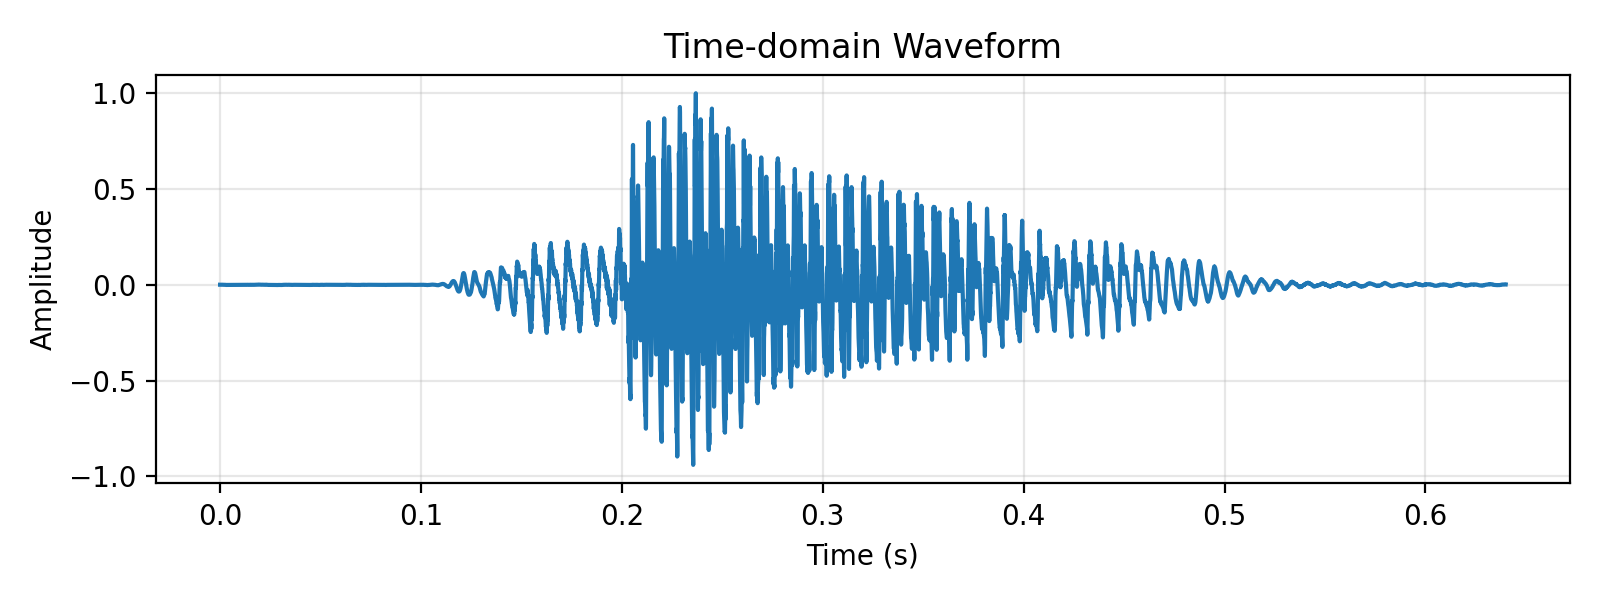
\includegraphics[width=0.75\linewidth]{signal_time_waveform.png}
  \caption{语音信号时域波形}
\end{figure}

\subsection{频域分析}

对离散语音信号作快速傅里叶变换（FFT），可得到其整体频率能量分布。离散傅里叶变换定义为
\begin{equation}
  X[k] = \sum_{n=0}^{N-1} x[n] e^{-j2\pi kn/N}.
\end{equation}

频谱图能够反映语音信号的主要频率成分和共振峰分布，但由于语音信号是典型非平稳信号，整体 FFT 无法表示频谱随时间的动态变化。

\begin{figure}[H]
  \centering
  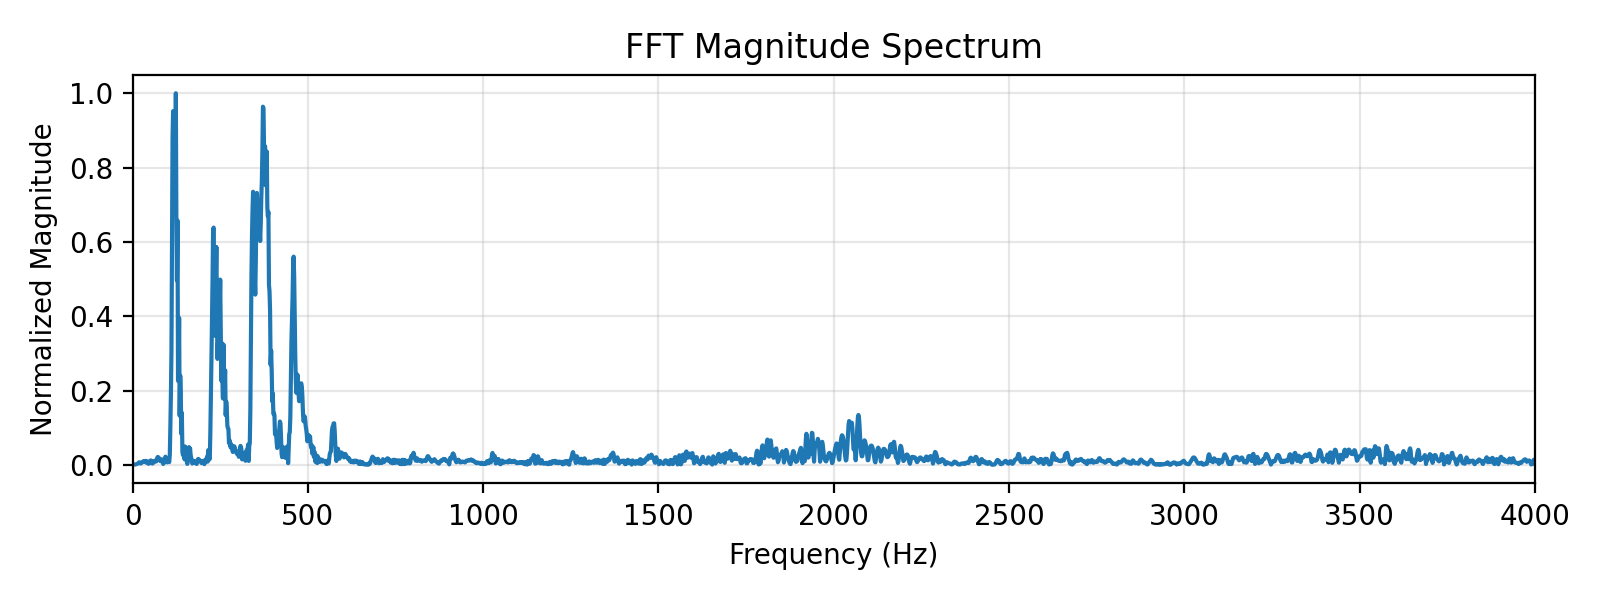
\includegraphics[width=0.75\linewidth]{signal_fft.png}
  \caption{语音信号 FFT 幅度谱}
\end{figure}

\subsection{短时傅里叶变换与语谱图}

为分析语音信号的时变频谱特性，实验采用短时傅里叶变换（STFT）。其基本思想是对信号进行分帧和加窗，在每一短时帧内近似认为信号平稳，再分别进行傅里叶变换：
\begin{equation}
  X(m,k)=\sum_{n=0}^{N-1} x[n]w[n-m]e^{-j2\pi kn/N}.
\end{equation}

本实验采用 25 ms Hamming 窗和 10 ms 帧移。语谱图横轴为时间，纵轴为频率，颜色表示能量强弱，可以同时展示语音的时间、频率和能量变化。

\begin{figure}[H]
  \centering
  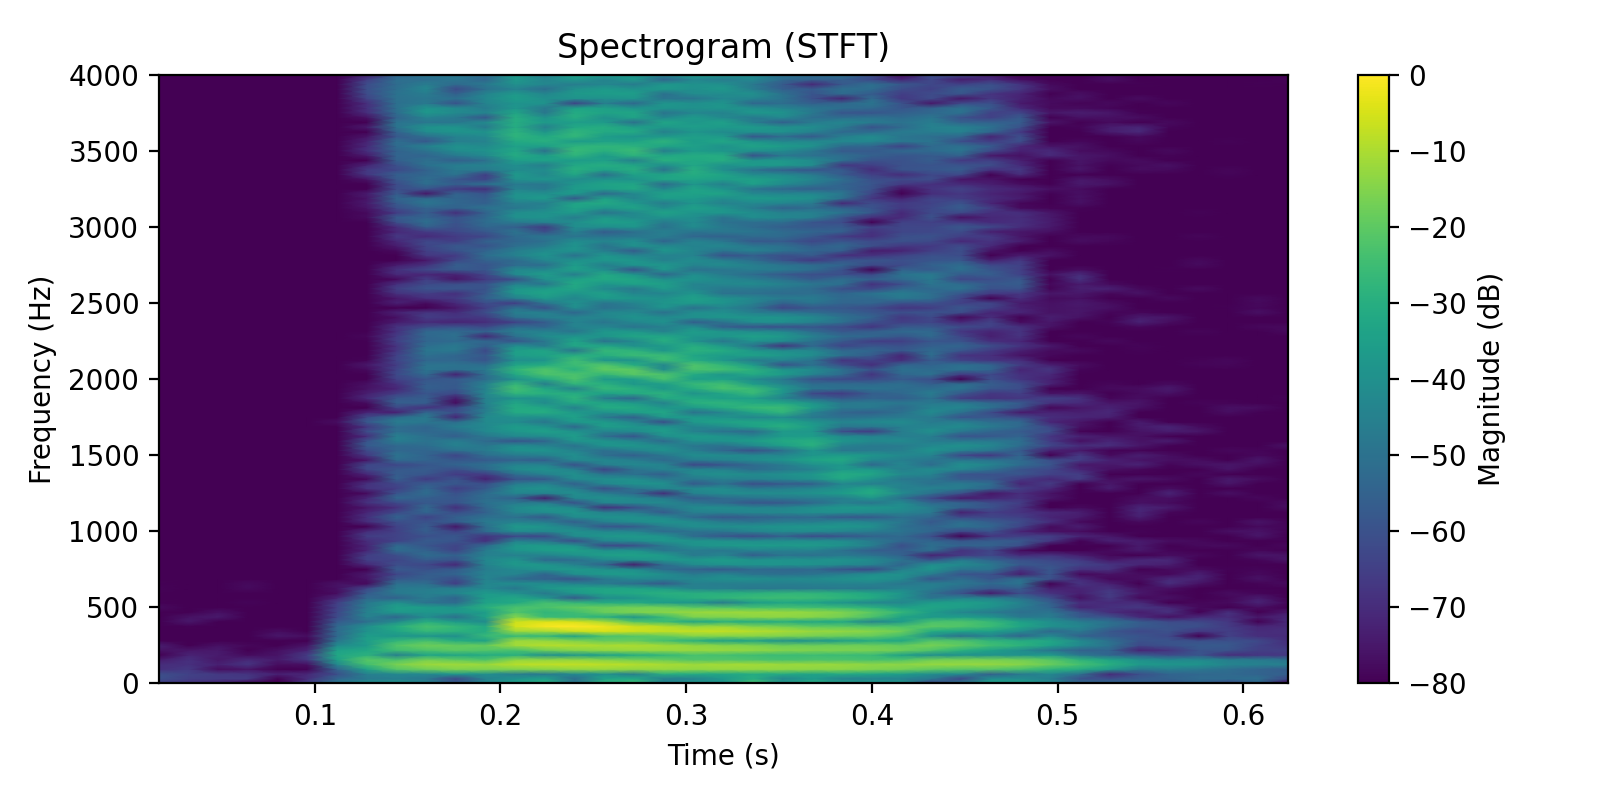
\includegraphics[width=0.75\linewidth]{signal_stft.png}
  \caption{语音信号 STFT 语谱图}
\end{figure}

\section{特征提取}

语音信号经过预处理和短时分析后，需要进一步提取能够表征不同数字之间声学差异的特征。
梅尔频率倒谱系数（Mel-Frequency Cepstral Coefficients, MFCC）是语音识别中最广泛应用的特征之一，
其设计模拟了人耳对声音的非线性感知特性。
本节详细介绍 MFCC 特征提取的完整流程，包括预加重、分帧加窗、FFT 与功率谱、梅尔滤波、对数压缩与离散余弦变换，以及动态特征的构建。

\subsection{预加重}

语音信号在唇辐射和空气传输过程中，高频分量会自然衰减。
为补偿这一效应，首先对离散语音信号 $x[n]$ 进行预加重（pre-emphasis），即通过一阶 FIR 高通滤波器：
\begin{equation}
  y[n] = x[n] - \alpha\,x[n-1],
\end{equation}
其中预加重系数 $\alpha = 0.97$。
该滤波器的作用是增强信号的高频成分，使频谱在高频段更加平坦，有利于后续的频谱分析。
从信号与系统的角度看，该系统的传递函数为 $H(z) = 1 - \alpha z^{-1}$，是一个简单的一阶高通 FIR 滤波器。

\subsection{分帧、加窗与短时傅里叶变换}

语音信号是典型的非平稳信号，其统计特性随时间变化。
但在较短的时段（约 20--30 ms）内，发音器官的运动相对缓慢，信号可近似视为平稳。
基于这一短时平稳假设，对预加重后的信号进行分帧处理：采用窗长为 25 ms 的 Hamming 窗，帧移为 10 ms。
在 16 kHz 采样率下，窗长对应 $N = 400$ 个采样点，帧移对应 $160$ 个采样点。

Hamming 窗的时域表达式为
\begin{equation}
  w[n] = 0.54 - 0.46\cos\left(\frac{2\pi n}{N-1}\right),\quad 0 \le n \le N-1.
\end{equation}
加窗可以减小帧边界处的不连续性，抑制频谱泄漏。

对每一帧加窗后的信号进行 $K$ 点 FFT，得到短时幅度谱 $|X(m,k)|$，进而计算功率谱 $|X(m,k)|^2$。
关于 STFT 的详细讨论见语音信号分析一节。

\subsection{梅尔滤波器组}

人耳对声音频率的感知是非线性的：在低频区域，人耳能够分辨较细微的频率差异；而在高频区域，频率分辨率则相对较低。
梅尔（Mel）尺度正是为了模拟这一感知特性而提出的一种频率映射，其与物理频率 $f$（Hz）的近似关系为
\begin{equation}
  \mathrm{Mel}(f) = 2595\log_{10}\!\left(1 + \frac{f}{700}\right).
\end{equation}

在梅尔尺度上等间距地放置一组三角滤波器，再映射回线性频率轴，即构成梅尔滤波器组。
梅尔滤波器在低频段分布密集、在高频段分布稀疏，体现了人耳的非线性频率分辨率。

本实验采用 40 个三角梅尔滤波器，频率范围为 20 Hz 至 7600 Hz（对应 16 kHz 采样的奈奎斯特频率以下）。
每一帧的功率谱通过梅尔滤波器组后，得到 40 维的对数梅尔能量。

\subsection{对数压缩与离散余弦变换}

将梅尔滤波器组的输出取对数，一方面模拟人耳对响度的对数感知特性，另一方面压缩动态范围，使特征对输入能量的绝对大小不敏感：
\begin{equation}
  S(m, l) = \log\left(\sum_{k=0}^{K-1} |X(m,k)|^2 \cdot H_l[k]\right),
\end{equation}
其中 $H_l[k]$ 为第 $l$ 个梅尔滤波器的频率响应，$l = 0, 1, \dots, L-1$，$L = 40$。

对数梅尔能量各维度之间存在较强的相关性。为降低特征维度并去除相关性，对 $S(m, l)$ 沿滤波器轴进行离散余弦变换（DCT）：
\begin{equation}
  c(m, i) = \sum_{l=0}^{L-1} S(m, l) \cos\!\left[\frac{\pi i}{L}\left(l + \frac{1}{2}\right)\right],\quad i = 0, 1, \dots, N_{\mathrm{mfcc}}-1.
\end{equation}
DCT 是一种正交变换，能够将能量集中到少数低阶系数上，同时使各阶倒谱系数近似不相关。
保留前 $N_{\mathrm{mfcc}} = 13$ 个 DCT 系数，即为该帧的 MFCC 特征。

值得注意的是，第 0 阶系数 $c(m,0)$（常记为 C0）主要反映该帧的整体能量，数值通常远大于其余系数。
在后续特征可视化中，为避免 C0 掩盖其他倒谱系数的细节结构，13 维 MFCC 图在绘制时省略 C0，仅显示 C1--C12。

\begin{figure}[H]
  \centering
  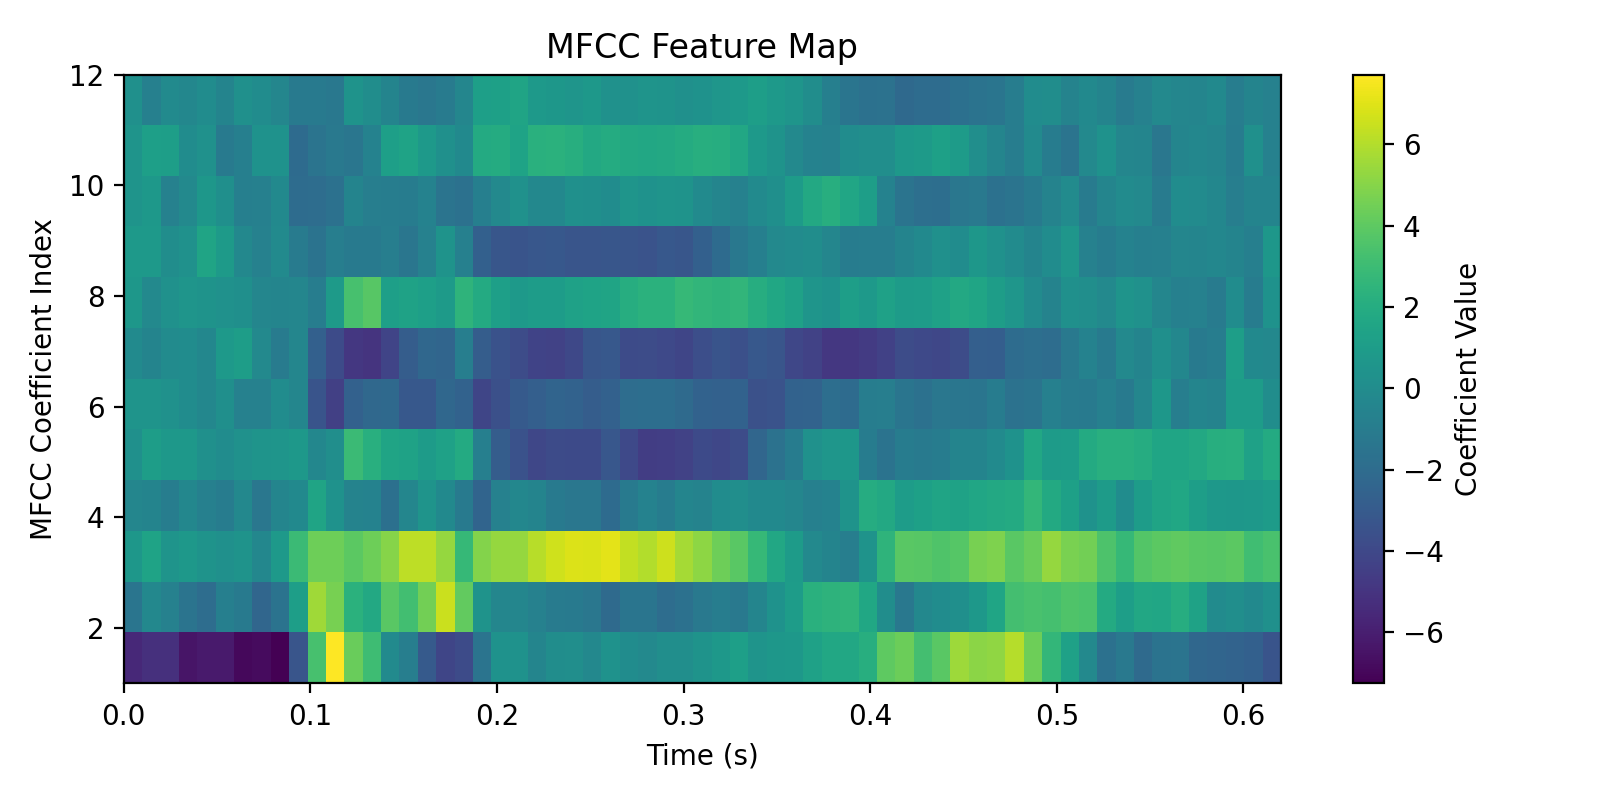
\includegraphics[width=0.75\linewidth]{signal_mfcc.png}
  \caption{13 维 MFCC 特征图（可视化时省略 C0，仅显示 C1--C12）。横轴为帧序号，纵轴为 MFCC 系数阶数，颜色表示系数值的大小。}
  \label{fig:mfcc13}
\end{figure}

\subsection{动态特征}

静态 MFCC 仅反映当前帧的频谱包络信息，无法刻画语音信号随时间变化的动态特性。
为此，在 13 维静态 MFCC 的基础上，分别计算一阶差分（Delta, $\Delta$）和二阶差分（Delta-Delta, $\Delta^2$）：
\begin{equation}
  \Delta_t = \frac{\sum_{n=1}^{N_d} n\,(c_{t+n} - c_{t-n})}{2\sum_{n=1}^{N_d} n^2},
\end{equation}
其中 $c_t$ 为第 $t$ 帧的 MFCC 向量，$N_d$ 为差分窗口半径（本实验取 $N_d = 2$）。
$\Delta^2$ 以同样的方式在 $\Delta$ 序列上计算得到。

最终，每一帧的特征向量由 13 维静态 MFCC、13 维 $\Delta$ 和 13 维 $\Delta^2$ 拼接而成，共计 39 维帧级特征。
动态特征的引入使模型能够同时利用频谱包络的静态信息和帧间变化的动态信息，从而更好地建模语音的时序演变规律。

\begin{figure}[H]
  \centering
  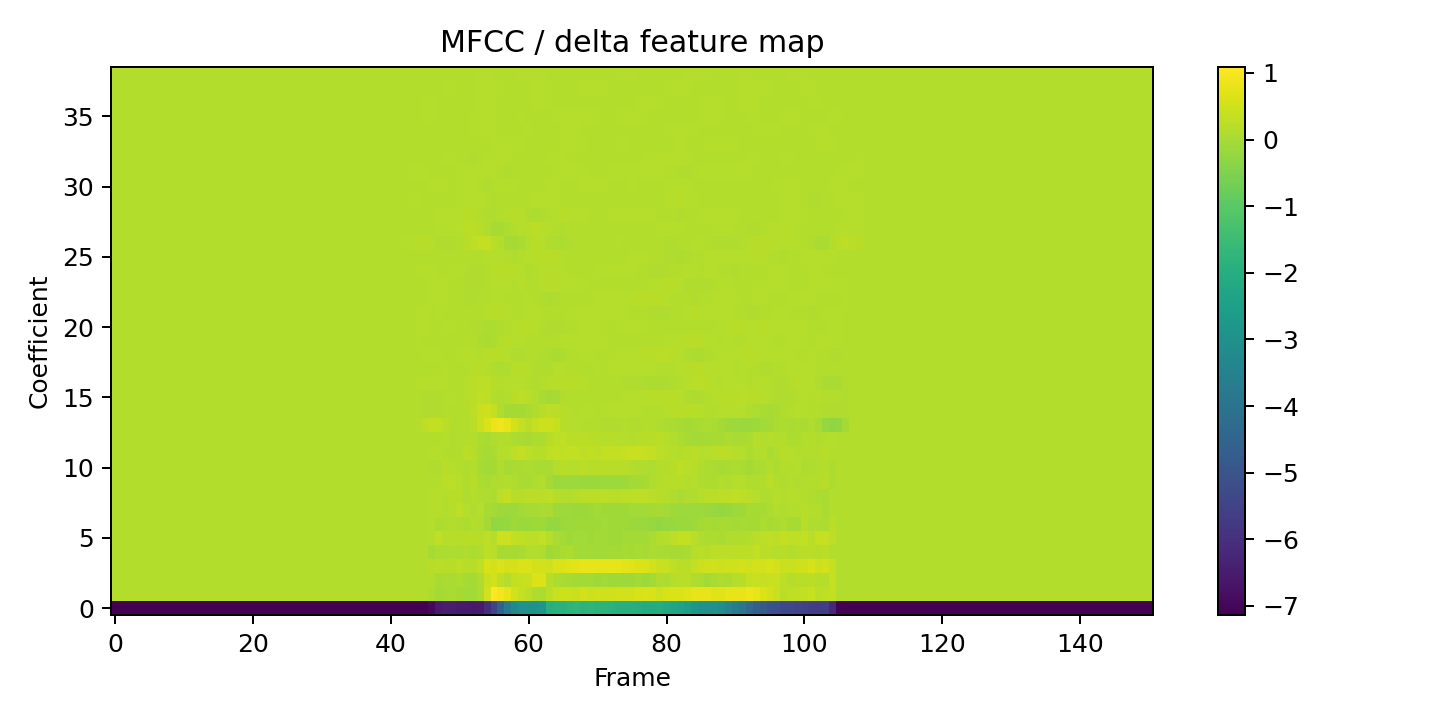
\includegraphics[width=0.75\linewidth]{signal_mfcc_features.png}
  \caption{39 维 MFCC + $\Delta$ + $\Delta^2$ 特征图。上段为 13 维静态 MFCC（含 C0），中段为 13 维 $\Delta$，下段为 13 维 $\Delta^2$。横轴为帧序号，纵轴为系数阶数。}
  \label{fig:mfcc39}
\end{figure}

图 \ref{fig:mfcc13} 和图 \ref{fig:mfcc39} 分别展示了同一语音段在两种特征表示下的可视化结果。
13 维特征图（图 \ref{fig:mfcc13}）聚焦于静态频谱包络的时变模式，不同数字的 MFCC 在特定系数阶数上呈现出差异化的能量分布；
39 维特征图（图 \ref{fig:mfcc39}）则进一步整合了动态信息，$\Delta$ 和 $\Delta^2$ 分量反映了频谱变化的速率与加速度，
为后续的分类模型提供了更丰富的时序判别依据。

\subsection{与信号与系统课程的关联}

MFCC 特征提取流程与信号与系统课程的知识体系紧密相关。
预加重对应一阶 FIR 滤波器的设计与频率响应分析；
分帧加窗涉及信号截断与频谱泄漏问题，是离散时间信号处理的重要内容；
FFT 和功率谱估计是频域分析的核心工具，在语音信号分析一节中已有详细讨论；
梅尔滤波器组体现了频域加权的思想，本质上是对功率谱的频域滤波；
对数运算实现动态范围压缩，与信号的非线性变换相关；
DCT 作为正交变换，具有能量集中和去相关的优良性质，是信号表示理论中的典型方法。
这些信号处理技术的有机结合，构成了从原始语音波形到紧凑声学特征表示的关键桥梁。

\section{分类方法}

\subsection{MFCC 统计特征 + KNN（Baseline）}

% TODO: baseline KNN method part

\subsection{MFCC 动态序列特征 + GMM}

针对 baseline 方法中``均值/方差''统计压缩丢失时序信息的问题，
本方法保留了语音的帧级时序结构，将每段语音建模为变长特征序列
$\{\mathbf{x}_1, \mathbf{x}_2, \ldots, \mathbf{x}_T\}$，其中
$\mathbf{x}_t \in \mathbb{R}^{39}$，$T$ 为帧数。
在此基础上，采用高斯混合模型（Gaussian Mixture Model, GMM）
作为分类器，从概率密度建模的角度直接处理变长序列。

\subsubsection{39 维动态特征提取}

仅使用 13 维静态 MFCC 只能描述当前帧的瞬时频谱包络，无法刻画语音信号的动态变化趋势。
为此，在静态 MFCC 的基础上引入一阶差分（$\Delta$）和二阶差分（$\Delta^2$）系数。

一阶差分 $\Delta$ 通过线性回归计算第 $t$ 帧附近 $N$ 帧窗口内的斜率，近似该帧处特征的一阶时间导数：

\begin{equation}
  \Delta_t = \frac{\sum_{i=1}^{N} i \cdot (\mathbf{c}_{t+i} - \mathbf{c}_{t-i})}{2 \sum_{i=1}^{N} i^2}
\end{equation}

其中 $\mathbf{c}_t$ 为第 $t$ 帧的 13 维 MFCC 向量，$N = 2$ 为上下文窗口宽度。
该公式对窗口内每条差分给予与距离成正比的权重，距离越远的帧对斜率估计贡献越大。

二阶差分 $\Delta^2$ 将一阶差分 $\Delta$ 再次通过同一回归公式计算得到，
近似二阶时间导数，反映频谱变化的``加速度''。最终将三者沿特征维度拼接：

\begin{equation}
  \mathbf{x}_t = \bigl[\,\mathrm{MFCC}_t \;\big|\; \Delta_t \;\big|\; \Delta^2_t \,\bigr] \in \mathbb{R}^{39}
\end{equation}

其中 MFCC$_t$ 为 13 维静态系数，$\Delta_t$ 为 13 维一阶差分，$\Delta^2_t$ 为 13 维二阶差分。
39 维特征同时编码了当前帧的频谱形状、变化速度和变化加速度，
为后续 GMM 提供了更丰富的声学判别信息。

\subsubsection{倒谱均值方差归一化（CMVN）}

不同说话人或不同录音条件下的信道差异会使 MFCC 分布发生整体偏移和尺度变化。
为降低此类变异对分类的影响，在提取 39 维特征后，
对每句语音逐维度进行基于句子的均值方差归一化（Cepstral Mean and Variance Normalization, CMVN）：

\begin{equation}
  \hat{\mathbf{x}}_t^{(d)} = \frac{\mathbf{x}_t^{(d)} - \mu^{(d)}}{\sigma^{(d)} + \varepsilon},\quad
  \mu^{(d)} = \frac{1}{T}\sum_{t=1}^{T} \mathbf{x}_t^{(d)},\quad
  \sigma^{(d)} = \sqrt{\frac{1}{T}\sum_{t=1}^{T} (\mathbf{x}_t^{(d)} - \mu^{(d)})^2}
\end{equation}

其中 $d = 1, \ldots, 39$ 为特征维索引，$\varepsilon = 10^{-8}$ 防止除零。
CMVN 使每维特征在句内均值为零、方差为一，有助于消除信道卷积噪声的线性滤波效应，
并减小不同说话人之间的特征分布差异。

\subsubsection{GMM 分类器}

高斯混合模型将数据分布建模为 $K$ 个高斯分量的加权和。
对于数字类别 $c \in \{0, 1, \ldots, 9\}$，独立训练一个 GMM，
其概率密度函数为：

\begin{equation}
  p(\mathbf{x} \mid \lambda_c) = \sum_{k=1}^{K} w_{c,k} \,
  \mathcal{N}\bigl(\mathbf{x} \mid \bm{\mu}_{c,k}, \bm{\Sigma}_{c,k}\bigr)
\end{equation}

其中 $w_{c,k}$ 为第 $k$ 个分量的混合权重（$\sum_k w_{c,k} = 1$），
$\bm{\mu}_{c,k}$ 为均值向量，$\bm{\Sigma}_{c,k}$ 为协方差矩阵。
本实验设定 $K = 4$ 个高斯分量，协方差类型为对角阵（\texttt{diag}），
兼顾模型容量与参数估计稳定性。

训练阶段，对每个数字类别 $c$，将该类所有训练样本的全部帧拼接为训练集
$X_c = \{\mathbf{x}^{(1)}, \mathbf{x}^{(2)}, \ldots, \mathbf{x}^{(M_c)}\}$，
通过期望最大化（EM）算法迭代估计 GMM 参数 $\lambda_c = \{w_{c,k}, \bm{\mu}_{c,k}, \bm{\Sigma}_{c,k}\}_{k=1}^{K}$。

预测阶段，对于测试样本的特征序列 $X = \{\mathbf{x}_1, \ldots, \mathbf{x}_T\}$，
假设各帧独立同分布，计算该序列在每个类 GMM 下的平均对数似然：

\begin{equation}
  \log p(X \mid \lambda_c) = \frac{1}{T} \sum_{t=1}^{T}
  \log \sum_{k=1}^{K} w_{c,k} \, \mathcal{N}(\mathbf{x}_t \mid \bm{\mu}_{c,k}, \bm{\Sigma}_{c,k})
\end{equation}

取对数似然最大的类别作为预测结果：
$\hat{y} = \arg\max_c \log p(X \mid \lambda_c)$。
与 KNN 仅比较样本间距离不同，GMM 从概率生成模型的角度
显式建模每类语音的帧级特征分布，能够更充分地利用时序特征的统计信息。

\subsubsection{与 Baseline 方法的对比}

表~\ref{tab:method_comparison} 总结了 Advanced GMM 方法与 baseline KNN 方法的主要区别。

\begin{table}[H]
  \centering
  \caption{Baseline KNN 与 Advanced GMM 方法对比}
  \label{tab:method_comparison}
  \begin{tabular}{@{}p{3.2cm} p{5.5cm} p{5.5cm}@{}}
    \toprule
    维度 & Baseline KNN & Advanced GMM \\
    \midrule
    特征维度 & 13 维 MFCC & 39 维（MFCC + $\Delta$ + $\Delta^2$） \\
    \addlinespace
    时序处理 & 均值/方差压缩为 26 维定长向量，丢弃时序 & 保留全部帧序列 $(T, 39)$ \\
    \addlinespace
    归一化 & StandardScaler（全局） & CMVN（逐句均值方差归一化） \\
    \addlinespace
    分类器 & 1-NN（基于欧氏距离） & GMM（$K=4$，对角协方差，对数似然评分） \\
    \addlinespace
    决策依据 & 最近邻样本标签 & 各类别概率密度建模 \\
    \bottomrule
  \end{tabular}
\end{table}

\section{实验结果与噪声鲁棒性分析}

本节对三种识别方法在纯净语音和混合噪声条件下的实验结果进行比较。
纯净语音实验用于评估模型在理想条件下的基本分类能力；噪声鲁棒性实验则通过在验证集语音中叠加不同强度的混合噪声，考察识别系统在实际复杂环境下的稳定性。

\subsection{纯净语音识别结果}

在无噪声条件下，三种方法均使用 speaker 6--7 的 20 条验证语音进行测试。
表 \ref{tab:clean-result-compare} 总结了三种方法的输入特征与识别准确率。
其中，KNN 使用 13 维 MFCC 的均值和标准差构成 26 维统计特征；GMM 使用 39 维 MFCC + $\Delta$ + $\Delta^2$ 帧级序列特征；CNN 则将同样的 39 维动态特征组织为二维特征图进行卷积分类。

\begin{table}[H]
  \centering
  \caption{纯净语音条件下三种识别方法的准确率比较}
  \label{tab:clean-result-compare}
  \begin{tabular}{lcc}
    \toprule
    方法 & 输入特征 & 准确率 \\
    \midrule
    MFCC-stat + KNN & 26 维统计特征 & 80.0\% \\
    MFCC + $\Delta$ + $\Delta^2$ + GMM & 39 维帧级序列特征 & 100.0\% \\
    TinyKeywordCNN & $39 \times T$ MFCC 动态特征图 & 100.0\% \\
    \bottomrule
  \end{tabular}
\end{table}

从结果可以看出，GMM 与 TinyKeywordCNN 在纯净语音条件下均达到 100.0\% 的验证准确率，20 条验证样本全部识别正确。
其中，GMM 说明在小样本条件下，用概率生成模型直接建模变长帧序列是有效的；CNN 则说明经过数据增强后，卷积网络能够从 MFCC 动态特征图中学习到有效的局部时频判别模式。
KNN 的准确率为 80.0\%，主要混淆包括 $0 \rightarrow 7$、$2 \rightarrow 8$、$4 \rightarrow 3$、$6 \rightarrow 9$，反映出均值/标准差统计池化会损失部分发音过程中的时间顺序信息。

\subsection{噪声添加方法与评价指标}

噪声鲁棒性测试中，保持训练好的模型参数不变，仅对验证集语音添加噪声后重新识别。
混合噪声由高斯白噪声、1/f 粉红噪声和 50 Hz 工频干扰组成。
其中，白噪声近似覆盖全频段，会整体抬高频谱噪声底；1/f 噪声能量更集中于低频区域，容易与语音中的低频共振峰重叠；50 Hz 工频干扰则对应实际采集系统中常见的窄带周期性干扰。

设干净语音为 $x[n]$，归一化后的混合噪声为 $v[n]$。
为了得到目标信噪比 $\mathrm{SNR}_{\mathrm{dB}}$，首先计算两者平均功率
\begin{equation}
  P_x=\frac{1}{N}\sum_{n=0}^{N-1}x^2[n],\qquad
  P_v=\frac{1}{N}\sum_{n=0}^{N-1}v^2[n].
\end{equation}
随后令噪声缩放系数为
\begin{equation}
  \alpha=\sqrt{\frac{P_x}{P_v\cdot 10^{\mathrm{SNR}_{\mathrm{dB}}/10}}},
\end{equation}
并构造带噪语音
\begin{equation}
  x_{\mathrm{noisy}}[n]=x[n]+\alpha v[n].
\end{equation}

KNN 与 GMM 在 $-10$ dB 至 20 dB 的 7 个 SNR 等级下测试，每个等级重复生成 20 次随机噪声，并统计识别准确率的均值和标准差。
CNN 使用更细的 mixed noise SNR 网格进行测试，SNR 范围扩展至 30 dB，用于观察数据增强后模型在不同噪声强度下的变化趋势。
由于 CNN 曲线不是 KNN/GMM 的同一套 20 次重复均值实验，因此下文主要比较趋势和最低可用 SNR，而不作严格统计显著性比较。

\subsection{KNN 基线的噪声鲁棒性}

图 \ref{fig:noise-knn} 给出了 KNN 基线在不同 SNR 下的识别准确率曲线。
可以看到，KNN 在带噪条件下性能下降明显。
当 SNR 较低时，准确率接近随机猜测水平；即使 SNR 提升到 20 dB，平均准确率也仅恢复到约 50\%，仍明显低于纯净语音下 80.0\% 的准确率。

\begin{figure}[H]
  \centering
  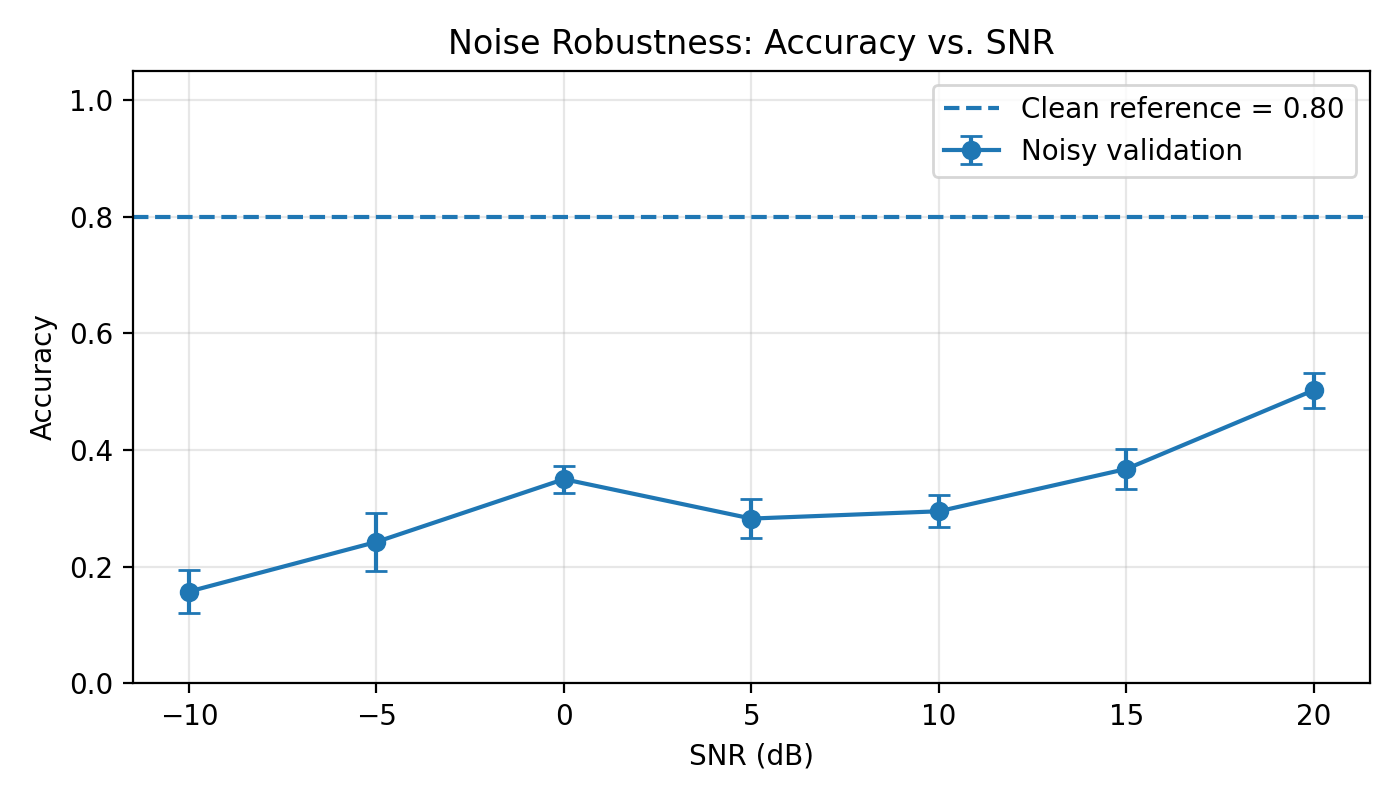
\includegraphics[width=0.72\linewidth]{noise_knn_accuracy_snr.png}
  \caption{KNN 基线在混合噪声下的准确率--SNR 曲线。曲线为 20 次重复实验的平均准确率，误差棒表示标准差。}
  \label{fig:noise-knn}
\end{figure}

造成这一现象的主要原因在于，KNN 所使用的均值/标准差统计特征对噪声扰动较为敏感。
噪声会改变各帧 MFCC 的整体分布，进而影响全局均值和标准差；同时，KNN 采用欧氏距离进行最近邻匹配，距离度量本身没有显式区分语音结构变化与噪声扰动。
因此，在带噪条件下，原本相近的同类样本可能被拉远，不同类样本也可能因噪声而意外接近，导致分类边界不稳定。

从最低可用 SNR 的角度看，在本实验设置的 $-10$ dB 至 20 dB 范围内，KNN 没有达到 90\% 以上准确率，说明其只能作为纯净或弱干扰条件下的简单基线，不适合作为主要鲁棒识别方案。

\subsection{GMM 序列模型的噪声鲁棒性}

图 \ref{fig:noise-gmm} 给出了 GMM 模型在混合噪声下的准确率--SNR 曲线，表 \ref{tab:noise-gmm} 给出了对应的 20 次重复均值与标准差。
与 KNN 相比，GMM 的性能随 SNR 提升呈现更加稳定的上升趋势。
在低 SNR 条件下，噪声仍会显著破坏 MFCC 特征，使模型难以可靠区分数字类别；但当 SNR 提升到中高区间后，GMM 的准确率提升明显，并在 20 dB 时达到 91.25\%。

\begin{table}[H]
  \centering
  \caption{GMM 在不同 SNR 下的噪声鲁棒性结果（20 次重复）}
  \label{tab:noise-gmm}
  \begin{tabular}{ccc}
    \toprule
    SNR (dB) & 平均准确率 & 标准差 \\
    \midrule
    $-10$ & 0.1000 & $1.39 \times 10^{-17}$ \\
    $-5$  & 0.1575 & 0.0426 \\
    $0$   & 0.3800 & 0.0731 \\
    $5$   & 0.5575 & 0.0729 \\
    $10$  & 0.7250 & 0.0433 \\
    $15$  & 0.8525 & 0.0460 \\
    $20$  & 0.9125 & 0.0311 \\
    \bottomrule
  \end{tabular}
\end{table}

\begin{figure}[H]
  \centering
  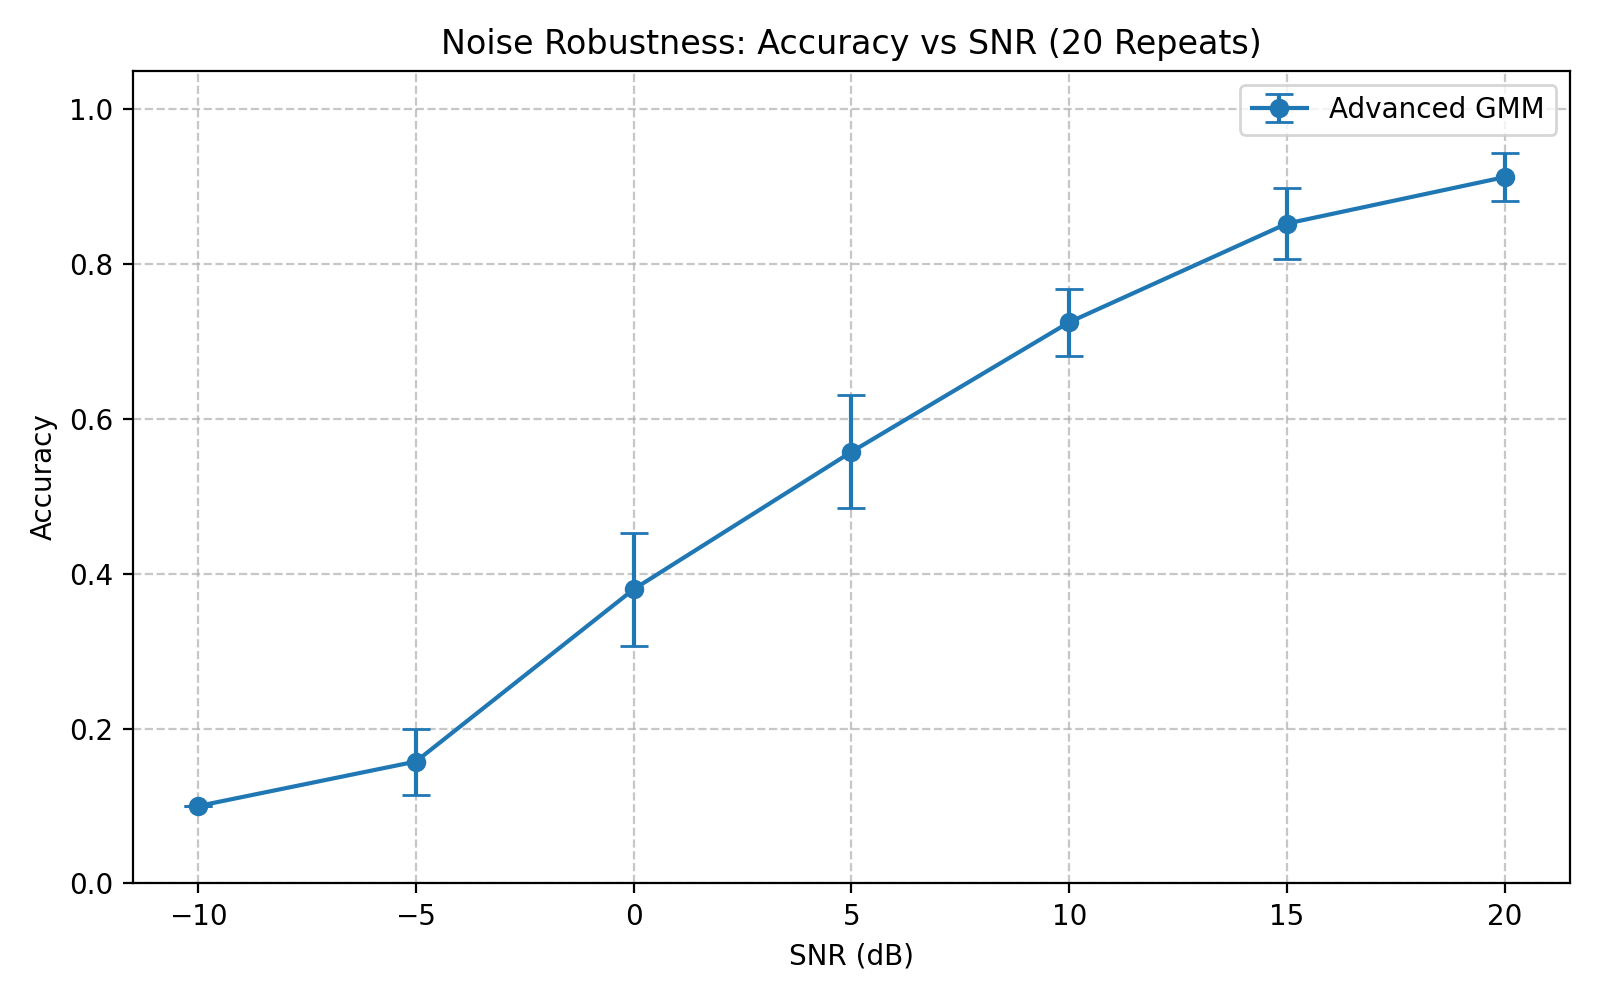
\includegraphics[width=0.72\linewidth]{noise_gmm_accuracy_snr.png}
  \caption{GMM 序列模型在混合噪声下的准确率--SNR 曲线。每个 SNR 重复 20 次，曲线展示平均准确率，误差棒表示标准差。}
  \label{fig:noise-gmm}
\end{figure}

GMM 相比 KNN 更鲁棒，主要有三方面原因。
第一，GMM 直接利用帧级序列特征，而不是将整段语音压缩为单一统计向量，因此保留了更多时间局部结构。
第二，MFCC + $\Delta$ + $\Delta^2$ 同时刻画频谱包络及其动态变化，使模型能够利用语音随时间演化的模式进行判别。
第三，CMVN 能够减小整体能量、信道和录音条件差异对倒谱特征的影响，从而在一定程度上削弱噪声造成的全局偏移。

根据实验结果，若以 90\% 准确率作为较高识别率标准，GMM 在测试范围内能够达到该标准的最低 SNR 为 20 dB。
这表明 GMM 是本实验传统方法中综合表现最稳定的方案，但在强噪声环境下仍存在明显性能下降。

\subsection{TinyKeywordCNN 的噪声鲁棒性}

图 \ref{fig:noise-cnn} 展示了 TinyKeywordCNN 在 mixed noise 条件下的准确率--SNR 曲线，表 \ref{tab:noise-cnn} 给出了对应的细粒度 SNR 测试结果。
与前一版结果相比，最终 CNN 训练配置加入了更强的噪声增强，并在纯净验证集上达到 100.0\%。
在带噪条件下，CNN 准确率随 SNR 提升整体上升：$-10$ dB 时准确率为 20\%，0 dB 时提升到 60\%，10 dB 时达到 85\%，并在 12.5 dB 首次达到 90\%；25 dB 时达到 100\%。

\begin{table}[H]
  \centering
  \caption{TinyKeywordCNN 在 mixed 噪声下不同 SNR 的识别准确率}
  \label{tab:noise-cnn}
  \small
  \begin{tabular}{ccccccccc}
    \toprule
    SNR/dB & $-10$ & $-7.5$ & $-5$ & $-2.5$ & $0$ & $2.5$ & $5$ & $7.5$ \\
    \midrule
    准确率/\% & 20 & 30 & 40 & 40 & 60 & 65 & 70 & 80 \\
    \bottomrule
  \end{tabular}

  \vspace{0.25cm}

  \begin{tabular}{ccccccccc}
    \toprule
    SNR/dB & $10$ & $12.5$ & $15$ & $17.5$ & $20$ & $22.5$ & $25$ & $30$ \\
    \midrule
    准确率/\% & 85 & 90 & 90 & 95 & 90 & 95 & 100 & 95 \\
    \bottomrule
  \end{tabular}
\end{table}

\begin{figure}[H]
  \centering
  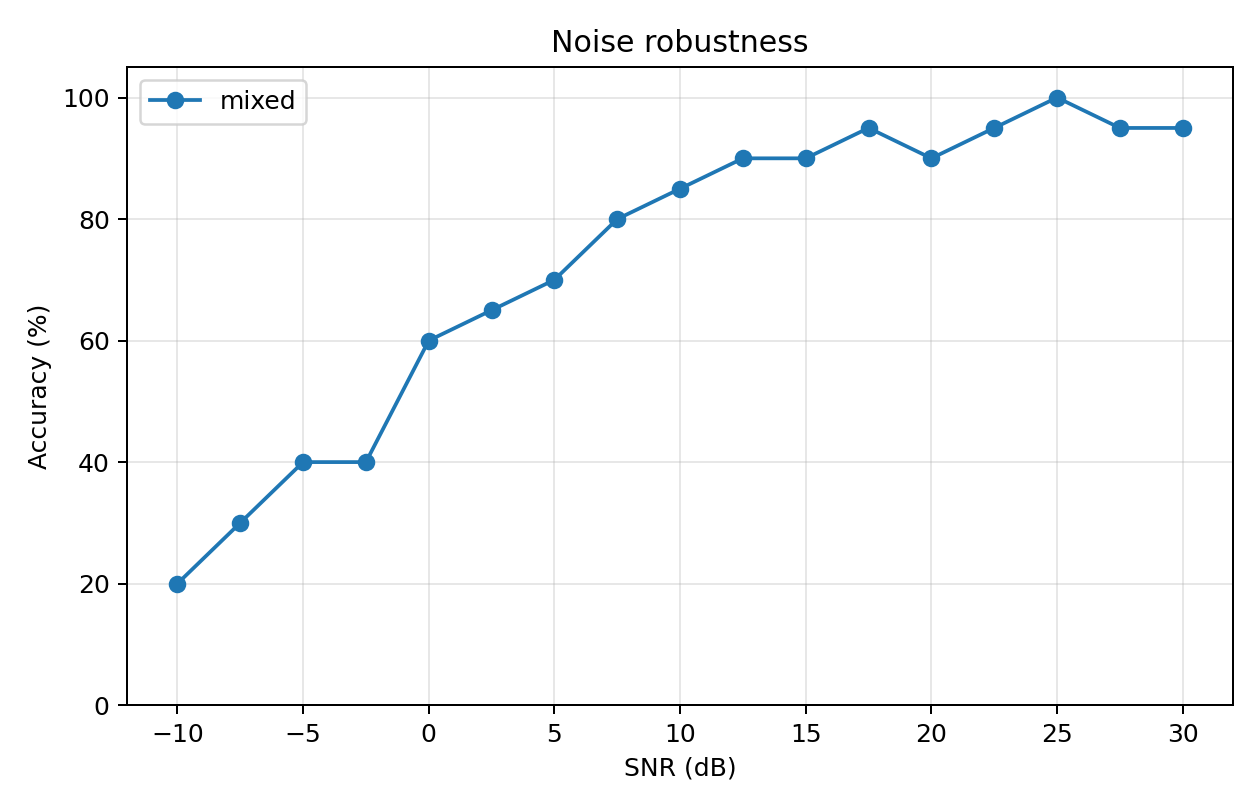
\includegraphics[width=0.72\linewidth]{noise_cnn_accuracy_snr.png}
  \caption{TinyKeywordCNN 在 mixed 噪声下的准确率--SNR 曲线。该曲线采用更细 SNR 网格，主要用于观察准确率随 SNR 变化的趋势。}
  \label{fig:noise-cnn}
\end{figure}

CNN 的优势在于能够通过卷积核学习 MFCC 特征图中的局部时频结构，而不是依赖人工定义的全局统计量或单帧概率密度。
同时，训练阶段加入了白噪声、粉红噪声和 50 Hz 工频干扰增强，使模型提前见到与鲁棒性测试相近的扰动形式，因此在中高 SNR 区间表现较好。
不过，由于本实验训练集仅有 50 条语音，验证集也仅有 20 条语音，CNN 的细粒度 SNR 曲线仍可能受到单次噪声抽样和小样本验证集的影响。
因此，本报告将 CNN 曲线主要作为深度学习路线的趋势参考，不将其与 KNN/GMM 的 20 次重复均值曲线作严格统计显著性比较。

\section{讨论与结论}

\subsection{各改进对识别性能的贡献分析}

\subsubsection{动态特征的贡献}

从 13 维静态 MFCC 扩展到 39 维动态特征（MFCC + $\Delta$ + $\Delta^2$）
是 Advanced GMM 方法性能提升的关键因素之一。
静态 MFCC 仅反映当前帧的瞬时频谱包络，
而 $\Delta$ 和 $\Delta^2$ 分别编码了频谱随时间变化的速度和加速度。
这些动态特征在语音识别中尤为重要，
因为不同数字的发音在共振峰过渡、能量上升/衰减速率等方面存在显著差异。
例如，数字``6''和``9''在静态 MFCC 空间中可能较为接近，
但它们的频谱变化轨迹不同——``6''的发音通常以低频能量逐步衰减为特征，
而``9''则涉及更复杂的共振峰运动——这些差异在动态特征空间中更容易被区分。

\subsubsection{CMVN 的贡献}

CMVN（倒谱均值方差归一化）在句子级别将每维特征归零均值、单位方差，
有效抑制了信道卷积噪声和说话人差异带来的线性频谱畸变。
与 baseline 中使用的全局 StandardScaler 不同，
CMVN 是逐句独立进行的，因此能够自适应地补偿不同句子的录制条件差异，
而不依赖训练集的整体统计量。
这一处理使分类器更关注语音内容的相对变化模式，而非绝对频谱值。

\subsubsection{GMM 概率建模的优势}

GMM 分类器相较于 KNN 的核心优势在于其概率生成建模的特性：
\begin{enumerate}[label=(\arabic*)]
  \item \textbf{时序信息保留}：GMM 直接对变长帧序列中的所有帧进行联合概率建模，
        而非像 KNN 那样将所有帧压缩为两个统计量（均值和方差）。
        这使得模型能够利用语音中丰富的帧级频谱分布信息；
  \item \textbf{类内分布建模}：每个 GMM 通过 4 个高斯分量近似该类语音在特征空间中的多模态分布。
        考虑到同一数字在不同上下文中、由不同说话人发出时，
        其声学特征可能呈现多种模式（如清辅音段、元音段、过渡段），
        多分量 GMM 能够自然地捕捉这种多模态性；
  \item \textbf{软判决与概率校准}：GMM 基于对数似然进行决策，
        其输出可以被解释为样本属于各类的相对置信度，
        比 KNN 的硬最近邻规则具有更好的泛化能力；
  \item \textbf{小样本鲁棒性}：在小样本（每类仅 5 个训练样本）条件下，
        GMM 通过对所有帧进行密度估计来利用全部可用数据，
        而 KNN 仅依赖少数几个训练样本的距离排序，更容易受到个别异常帧的影响。
\end{enumerate}

\subsection{噪声鲁棒性分析}

噪声实验结果表明，Advanced GMM 方法的性能随 SNR 下降呈现明显的退化趋势，
但退化程度相较 baseline 有明显改善。
以 \qty{20}{dB} SNR 为例，GMM 平均准确率为 0.9125，而 baseline 仅为 0.5025。

从现象层面分析，噪声对 GMM 的影响主要体现在以下方面：
\begin{enumerate}[label=(\arabic*)]
  \item 加性噪声改变了每一帧的功率谱形状，
        导致 MFCC 及其差分特征发生系统性偏移，
        使测试帧在 GMM 似然空间中的分布偏离训练分布；
  \item 在低 SNR（如 \qty{-10}{dB}）下，
        语音信号几乎被噪声淹没，提取的特征主要反映噪声特性而非语音内容，
        导致所有类别的对数似然趋近，分类退化为近似随机猜测（准确率 $\approx$ 0.10，与 10 类随机概率一致）；
  \item 噪声对 $\Delta$ 和 $\Delta^2$ 特征的影响尤为显著——高频噪声使相邻帧间出现大幅随机波动，
        导致差分特征的信噪比低于静态 MFCC，在低 SNR 下反可能成为干扰。
\end{enumerate}

值得注意的是，在 \qty{5}{dB} 至 \qty{20}{dB} 区间，
GMM 准确率随 SNR 单调提升且标准差较小（$< 0.075$），
表明该方法在该 SNR 范围内具有相对稳定的噪声鲁棒性。

\subsection{与 Baseline 方法的性能对比}

表~\ref{tab:comparison_baseline_gmm} 给出了 Baseline KNN 与 Advanced GMM 在纯净和不同噪声条件下的性能对比。

\begin{table}[H]
  \centering
  \caption{Baseline KNN 与 Advanced GMM 性能对比}
  \label{tab:comparison_baseline_gmm}
  \begin{tabular}{@{}cccc@{}}
    \toprule
    SNR & Baseline KNN 准确率 & Advanced GMM 准确率 & 提升幅度 \\
    \midrule
    Clean & 0.8000 & \textbf{1.0000} & $+0.2000$ \\
    \qty{20}{dB} & 0.5025 & \textbf{0.9125} & $+0.4100$ \\
    \qty{10}{dB} & 0.2950 & \textbf{0.7250} & $+0.4300$ \\
    \qty{0}{dB}  & 0.3500 & \textbf{0.3800} & $+0.0300$ \\
    \bottomrule
  \end{tabular}
\end{table}

可以看出，Advanced GMM 在所有条件下均优于 baseline，
尤其在中高 SNR（\qty{10}{dB}--\qty{20}{dB}）区间提升幅度最大（约 $+0.41$--$+0.43$）。
在 \qty{0}{dB} 及以下极端噪声条件下，两种方法的差距缩小，
说明当噪声强度超过语音信号本身时，特征提取本身成为瓶颈，
分类器的改进空间有限。

\subsection{局限性与改进方向}

尽管 Advanced GMM 方法在纯净和小噪声条件下表现出色，但仍存在以下局限：

\begin{enumerate}[label=(\arabic*)]
  \item \textbf{对角协方差假设}：为简化参数估计，
        本方法使用对角协方差矩阵（\texttt{diag}），
        假设 39 维特征各维之间相互独立。
        这一假设在实际中并不完全成立——
        MFCC 相邻维度之间以及 MFCC 与 $\Delta$/$\Delta^2$ 之间存在相关性。
        使用全协方差或 tied 协方差可能进一步提升性能；
  \item \textbf{高斯分量数固定}：$K = 4$ 是根据经验选取的，
        未对不同分量数进行系统调优。
        分量数过少可能不足以捕获类内多模态分布，
        过多则在小样本下容易过拟合；
  \item \textbf{小样本训练集}：每类仅 5 个训练样本，
        GMM 的 4 个分量共需估计 $4 \times (39 + 39) + 3 \approx 315$ 个参数（对角协方差下，含均值、方差与混合权重），
        训练数据量相对有限，可能导致参数估计不够精确；
  \item \textbf{缺少有效语音帧筛选}：当前方法将所有帧（包括低能量静音帧）纳入 GMM 建模。
        在加噪条件下，静音段被填充为纯噪声帧，其分布与训练集中的静音帧分布不同，
        可能拉低整体对数似然；
  \item \textbf{噪声场景单一}：噪声鲁棒性测试仅使用一种混合噪声类型，
        未评估对不同噪声类型（如语音 babble、街道噪声、音乐噪声等）的泛化能力。
\end{enumerate}

未来改进方向可包括：
(1) 引入语音活动检测（VAD），仅对有效语音帧进行 GMM 建模和评分；
(2) 使用 Bayesian Information Criterion（BIC）或交叉验证自动选择最优高斯分量数；
(3) 尝试全协方差 GMM 或结合 UBM（Universal Background Model）的自适应方法；
(4) 在特征层面引入噪声抑制或谱减法预处理，提高低 SNR 下的特征质量。

% --- End of GMM discussion subsection ---

\section{团队分工}

本实验由四名组员协作完成，整体工作包括数据预处理、语音信号分析、特征提取、传统机器学习模型、深度学习模型、噪声鲁棒性测试、结果可视化、报告撰写和展示材料整理。各成员在完成各自模块的基础上，也对整体实验流程、结果分析和报告修改进行了讨论与协作。

\begin{table}[H]
  \centering
  \caption{团队成员分工}
  \label{tab:team-contribution}
  \small
  \begin{tabular}{p{0.16\linewidth}p{0.76\linewidth}}
    \toprule
    成员 & 主要工作 \\
    \midrule
    于沛龙 &
    负责传统方法基线流程搭建，包括语音预处理、端点检测、MFCC 特征提取、KNN 基线模型实现与测试；参与噪声鲁棒性实验、结果图表整理、PPT 制作与实验报告统稿。 \\
    \addlinespace

    景序 &
    负责传统方法优化部分，设计并实现基于 MFCC + $\Delta$ + $\Delta^2$ 帧级特征的 GMM 序列模型；完成 GMM 纯净语音测试、噪声鲁棒性重复实验、准确率--SNR 曲线绘制及相关结果分析。 \\
    \addlinespace

    封宇凡 &
    负责深度学习方法部分，设计并训练 CNN 模型；完成 MFCC 动态特征图输入构建、网络结构设计、模型训练参数调优、纯净语音测试和混合噪声细粒度 SNR 测试。 \\
    \addlinespace

    孟德轩 &
    参与数据处理、实验结果核对、图表整理和报告材料撰写；协助完成实验流程梳理、不同方法结果对照、报告格式检查以及展示内容整理。 \\
    \bottomrule
  \end{tabular}
\end{table}

在协作过程中，小组首先确定整体技术路线：
以 MFCC 为核心声学特征，分别构建 KNN、GMM 和 CNN 三种识别方法，
并统一使用 speaker1--5 作为训练集、speaker6--7 作为验证集。
随后，各成员分别完成对应模型的实现与测试，并将输出结果统一整理为混淆矩阵、准确率表格和准确率--SNR 曲线。
最后，小组共同对实验结果进行比较分析，讨论不同方法在小样本条件和混合噪声条件下的优劣，完成最终实验报告和课程展示材料。


\newpage
\printbibliography

\end{document}
